%% read_data_formats.tex
%% Author: Leighton Pritchard
%% Copyright: James Hutton Institute
%% These slides briefly introduce the ways in which sequence 
%% data tends to arrive at the bioinformatician

% The two main current sequence read data formats
\begin{frame}
  \frametitle{What do you get from sequencing\footnote{\tiny{Miyamoto \textit{et al}. (2014) \textit{BMC Genomics} \textbf{15}:699 \href{http://dx.doi.org/10.1186/1471-2164-15-699}{doi:10.1186/1471-2164-15-699}}}}
  Sequence reads. Lots of them. \\
  Size/number depend on technology used.
    \begin{center}
      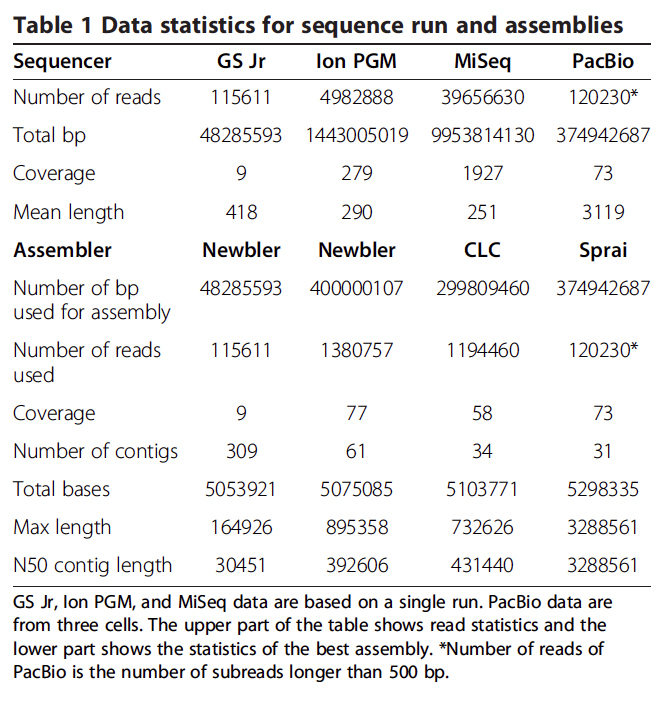
\includegraphics[height=0.7\textheight]{images/miyamoto_table}
    \end{center}   
\end{frame}

% The two main current sequence read data formats
\begin{frame}
  \frametitle{Sequence Read Data Formats}
  Two common read data sequence formats:
  \begin{itemize}
    \item \textbf{FASTQ}: Related to FASTA, a \textit{de facto} standard for sequence reads
    \item \textbf{SAM/BAM}: Sequence alignment/mapping format, two flavours - uncompressed and compressed
    \item \textbf{CRAM}: Reference-based sequence compression
  \end{itemize}
  You might also receive assembled genomes directly from a sequencing partner
\end{frame}

% SUBSECTION: FASTQ
% A very brief summary of the FASTQ format
\subsection{FASTQ}

% FASTQ data format
\begin{frame}[fragile]
  \frametitle{FASTQ\footnote{\tiny{\href{http://dx.doi.org/10.1093/nar/gkp1137}{Cock \textit{et al}. (2009) \textit{Bioinformatics} \textbf{38}:1767-1771 doi:10.1093/nar/gkp1137}}}}
\begin{verbatim}
@HISEQ2500-09:168:HA424ADXX:2:1101:1404:2061 1:N:0:ATCTCTCTCACCAACT
CGGTCTTGGGATAGATGGGTTGCAGGTTGCGGTAAAGCTCGGACTCCAGAGCGTCCAGGGTAGACTGGCTAATCTTCTGCTCTTTATCGATCATTATTTC
+
@@CBDDFFHHDFDHEGHIICGIFHHIIIIFHGGHIEHHIIIIGHGHIIIIIGGHHFFFFC@CBCCCDDBDCDDDDDDDDCCDDDD3@ABDDDDDEEEDE@
\end{verbatim}
  Files typically have \texttt{.fq}, \texttt{.fastq} extension. \\
  Four lines per sequence
  \begin{enumerate}
    \item Header: sequence identifier and optional description, starts with ``@''
    \item Raw sequence (\texttt{[ACGTN]})
    \item \textit{Optional} header, repeats line 1, starts with ``+''
    \item Quality scores, numbers encoded as ASCII
  \end{enumerate}
\end{frame}

% FASTQ data format
\begin{frame}[fragile]
  \frametitle{FASTQ encoding\footnote{\tiny{\href{http://dx.doi.org/10.1093/nar/gkp1137}{Cock \textit{et al}. (2009) \textit{Bioinformatics} \textbf{38}:1767-1771 doi:10.1093/nar/gkp1137}}}}
  More than one version of FASTQ, differ by quality encoding \\
  Numbers converted to ASCII start at different values
    \begin{center}
      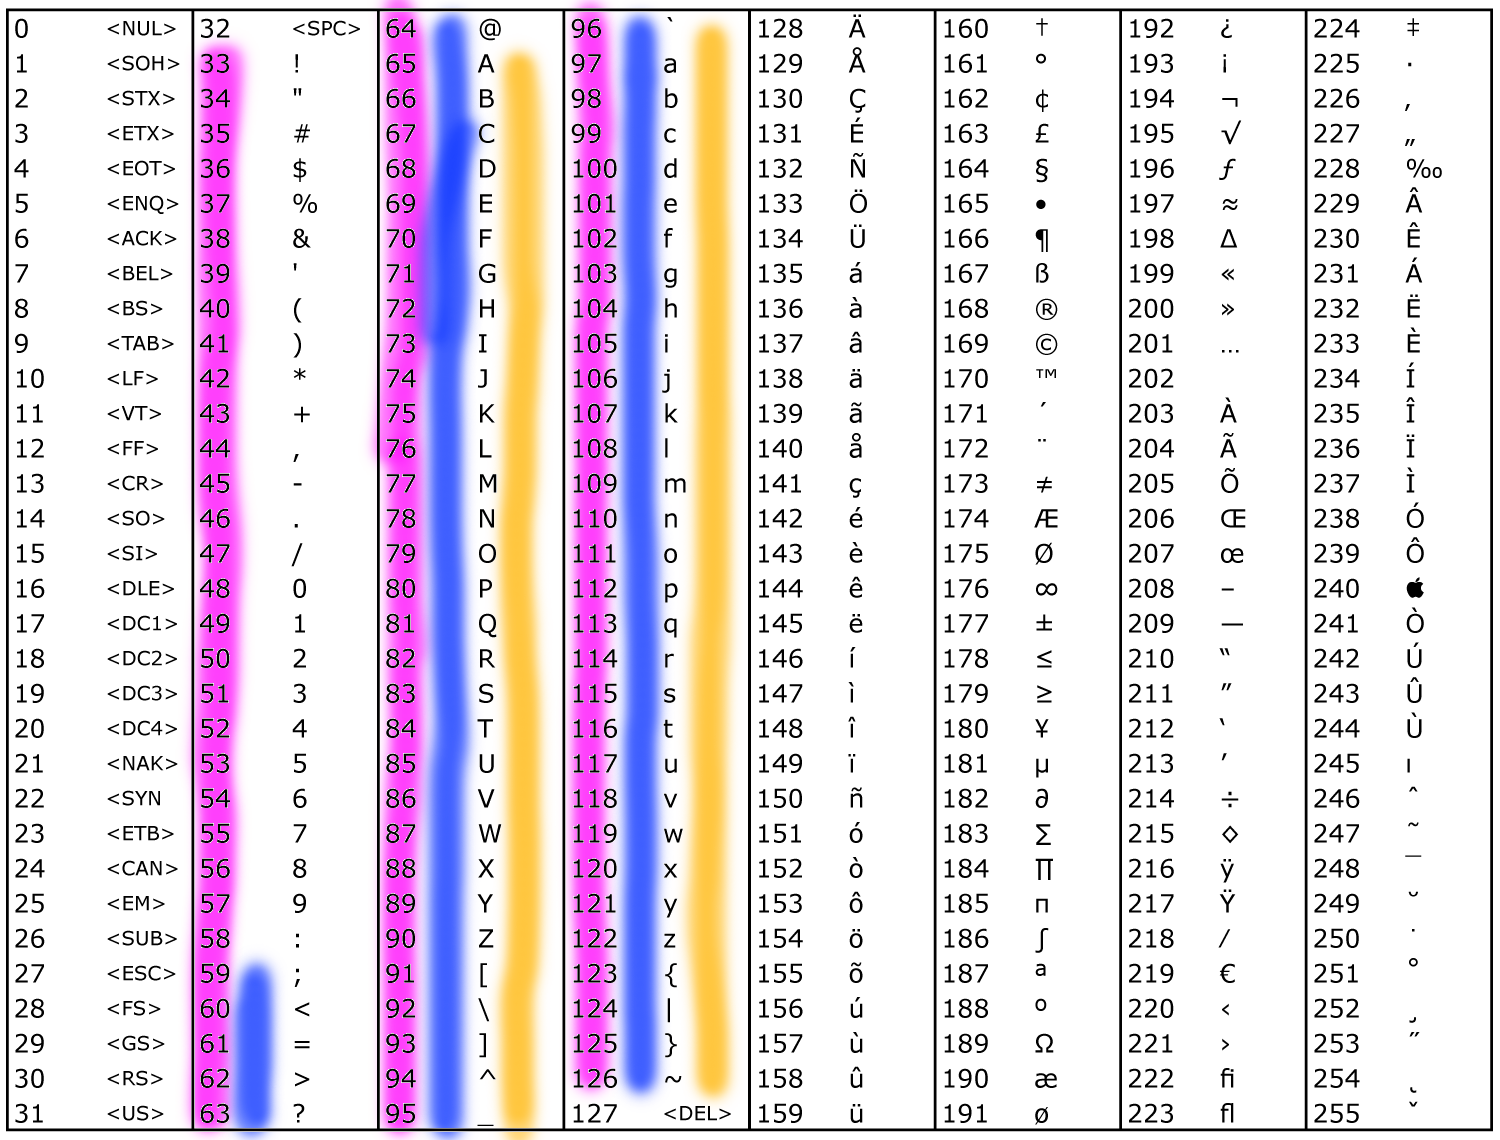
\includegraphics[height=0.7\textheight]{images/ascii_table}
    \end{center}  
\end{frame}

% FASTQ data format
\begin{frame}[fragile]
  \frametitle{FASTQ encoding\footnote{\tiny{\href{http://dx.doi.org/10.1093/nar/gkp1137}{Cock \textit{et al}. (2009) \textit{Bioinformatics} \textbf{38}:1767-1771 doi:10.1093/nar/gkp1137}}}}
  Versions vary by sequencer and period. Most now settled on Sanger format. \\
  Quality scores ($Q_{phred}$) offset to lie in the given range:
  \begin{enumerate}
    \item \textbf{Sanger}: 33-126, used in SAM/BAM, and Illumina 1.8+
    \item \textbf{Illumina 1.0-1.2}: 59-126
    \item \textbf{Illumina 1.3-1.8}: 64-126
  \end{enumerate}
  $Q_{phred} = -10 \log_{10}e$, where $e$ is the estimated probability that a base call is incorrect.
\end{frame}

% Variation in quality: good reads
\begin{frame}[fragile]
  \frametitle{Quality Control}
  The quality of basecalls varies along reads.\\
  \begin{center}
    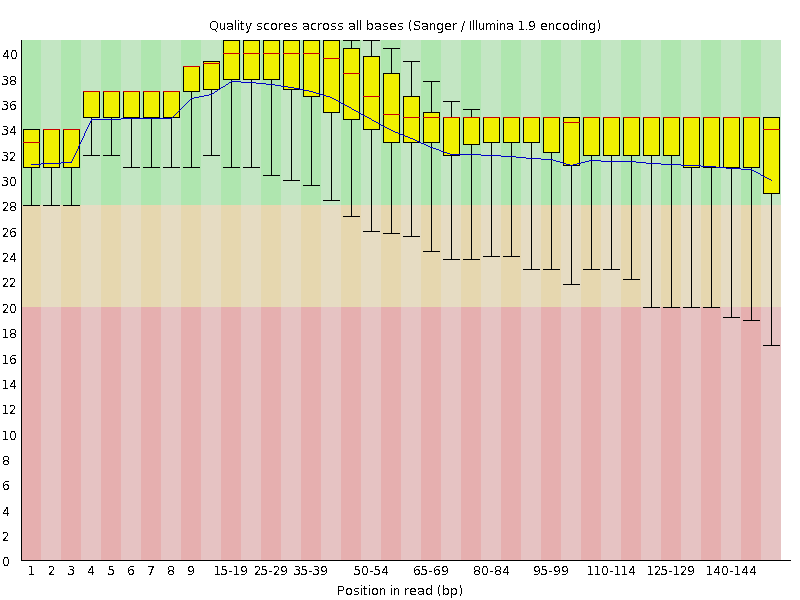
\includegraphics[height=0.6\textheight]{images/per_base_quality}
  \end{center}  
  (real data from our \textit{E.coli} sequencing: good quality)
\end{frame}

% Variation in quality: bad reads
\begin{frame}[fragile]
  \frametitle{Quality Control}
  Some datasets are better than others.\\
  \begin{center}
    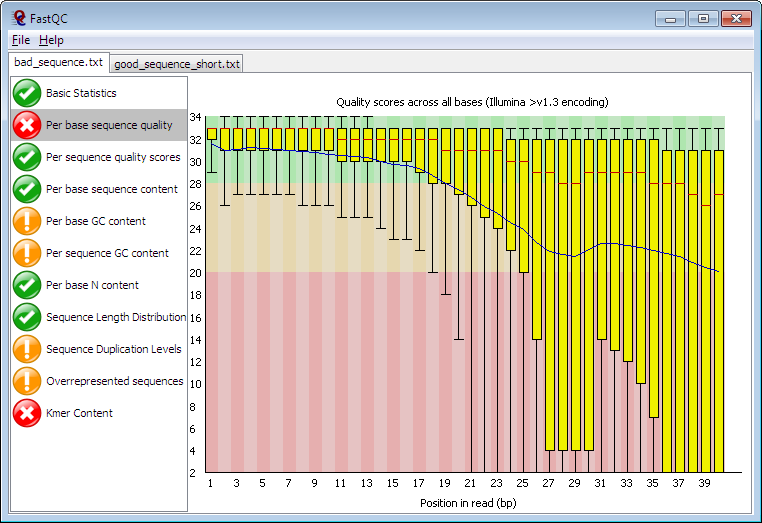
\includegraphics[height=0.5\textheight]{images/fastqc}
  \end{center}  
  Reads can be trimmed, or discarded.\\
  Including poor reads compromises assembly.
\end{frame}


% SUBSECTION: SAM/BAM/CRAM
% A very brief summary of the SAM/BAM/CRAM formats
\subsection{SAM/BAM/CRAM}

% SAM data format
\begin{frame}[fragile]
  \frametitle{SAM\footnote{\tiny{\href{http://samtools.github.io/hts-specs/SAMv1.pdf}{https://github.com/samtools/hts-specs}}}}
  \begin{center}
    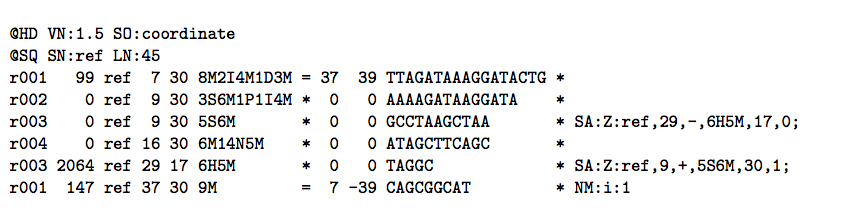
\includegraphics[width=0.8\textwidth]{images/sam_format}
  \end{center}  
  Intended to represent read alignments, also used for raw reads. \\
  Tab-delimited plain text. Headers (\textit{optional}) start with ``@'' \\
  \begin{center}
    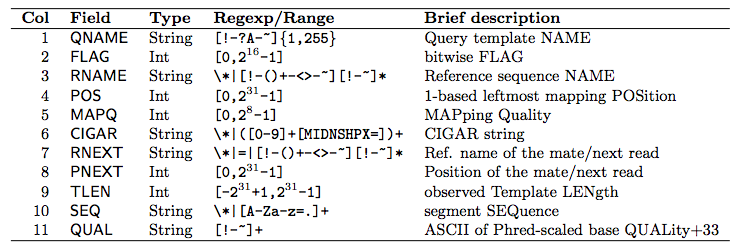
\includegraphics[width=0.8\textwidth]{images/sam_columns}
  \end{center}  
\end{frame}

% BAM data format
\begin{frame}[fragile]
  \frametitle{BAM\footnote{\tiny{\href{http://samtools.github.io/hts-specs/SAMv1.pdf}{https://github.com/samtools/hts-specs}}}/CRAM\footnote{\tiny{\href{http://www.ebi.ac.uk/ena/software/cram-toolkit}{http://www.ebi.ac.uk/ena/software/cram-toolkit}}}}
  BAM is a compressed version of SAM.\\
  \begin{itemize}
    \item BGZF compression.
    \item Random access within compressed file, through indexing.
  \end{itemize}
  CRAM format may come to dominate, especially in archives, as datasets get larger:
  \begin{itemize}
    \item Reference-based compression.\footnote{\tiny{\href{http://dx.doi.org/10.1101/gr.114819.110}{Fritz \textit{et al}. (2011) \textit{Genome Res.} \textbf{21}:734-740 doi:10.1101/gr.114819.110}}}
    \item Highly suited to compression and archiving of \textit{very} large amounts of sequence data.\footnote{\tiny{\href{http://dx.doi.org/10.1186/2047-217X-1-2}{Cochrane \textit{et al}. (2012) \textit{GigaScience} \textbf{1}:2 doi:10.1186/2047-217X-1-2}}}
  \end{itemize}  
\end{frame}

